\documentclass[superscriptaddress,onecolumn,floatfix]{revtex4-2}

\usepackage{graphicx}
\usepackage{epsfig}
\usepackage{color}
\usepackage{amssymb}
\usepackage{amsmath}
\usepackage{array}
\usepackage[loose]{units}
\usepackage[french]{babel}
\usepackage[unicode]{hyperref}
\usepackage{cleveref}
\usepackage{braket}
\usepackage[caption=false]{subfig}
\usepackage{letltxmacro}

\pdfcompresslevel=9

\LetLtxMacro{\ORIGselectlanguage}{\selectlanguage}
\makeatletter
\DeclareRobustCommand{\selectlanguage}[1]{%
    \@ifundefined{alias@\string#1}
      {\ORIGselectlanguage{#1}}
      {\begingroup\edef\x{\endgroup
         \noexpand\ORIGselectlanguage{\@nameuse{alias@#1}}}\x}%
}
\newcommand{\definelanguagealias}[2]{%
  \@namedef{alias@#1}{#2}%
}
\makeatother

\definelanguagealias{fr}{french}


\begin{document}
\selectlanguage{fr}

\begin{abstract}
  Ce guide vous guide à travers les étapes nécessaires pour installer le faisceau CAN sélectionnable dans votre Ioniq 5 2021-2024. Voir également le \href{https://youtube.com/playlist?list=PLYCTmVJH4UYqnw87UZAaqMo1GrOv0cJaL}{guides vidéo}:
  \begin{description}
    \item[Étape 1 : Débranchez le 12 V] \href{https://youtu.be/ePBdyeBYKk4}{guide vidéo}
    \item[Étape 2 : Installer le harnais] \href{https://youtu.be/kVvkR4ZLFMI}{guide d'installation du harnais}
  \end{description}
\end{abstract}
\title{Guide d'installation CAN sélectionnable}
\author{Boutique de boutons Electroniq}
\email{support@electroniqbuttons.com}
% \affiliation{\GOE}
% \author{Benjamin J. McMorran}
% \email{mcmorran@uoregon.edu}
% \affiliation{\UO}
\date{\today}

\maketitle

% \begin{figure}[h]
%   \subfloat[]{\label{subfig:overview:harness}
%   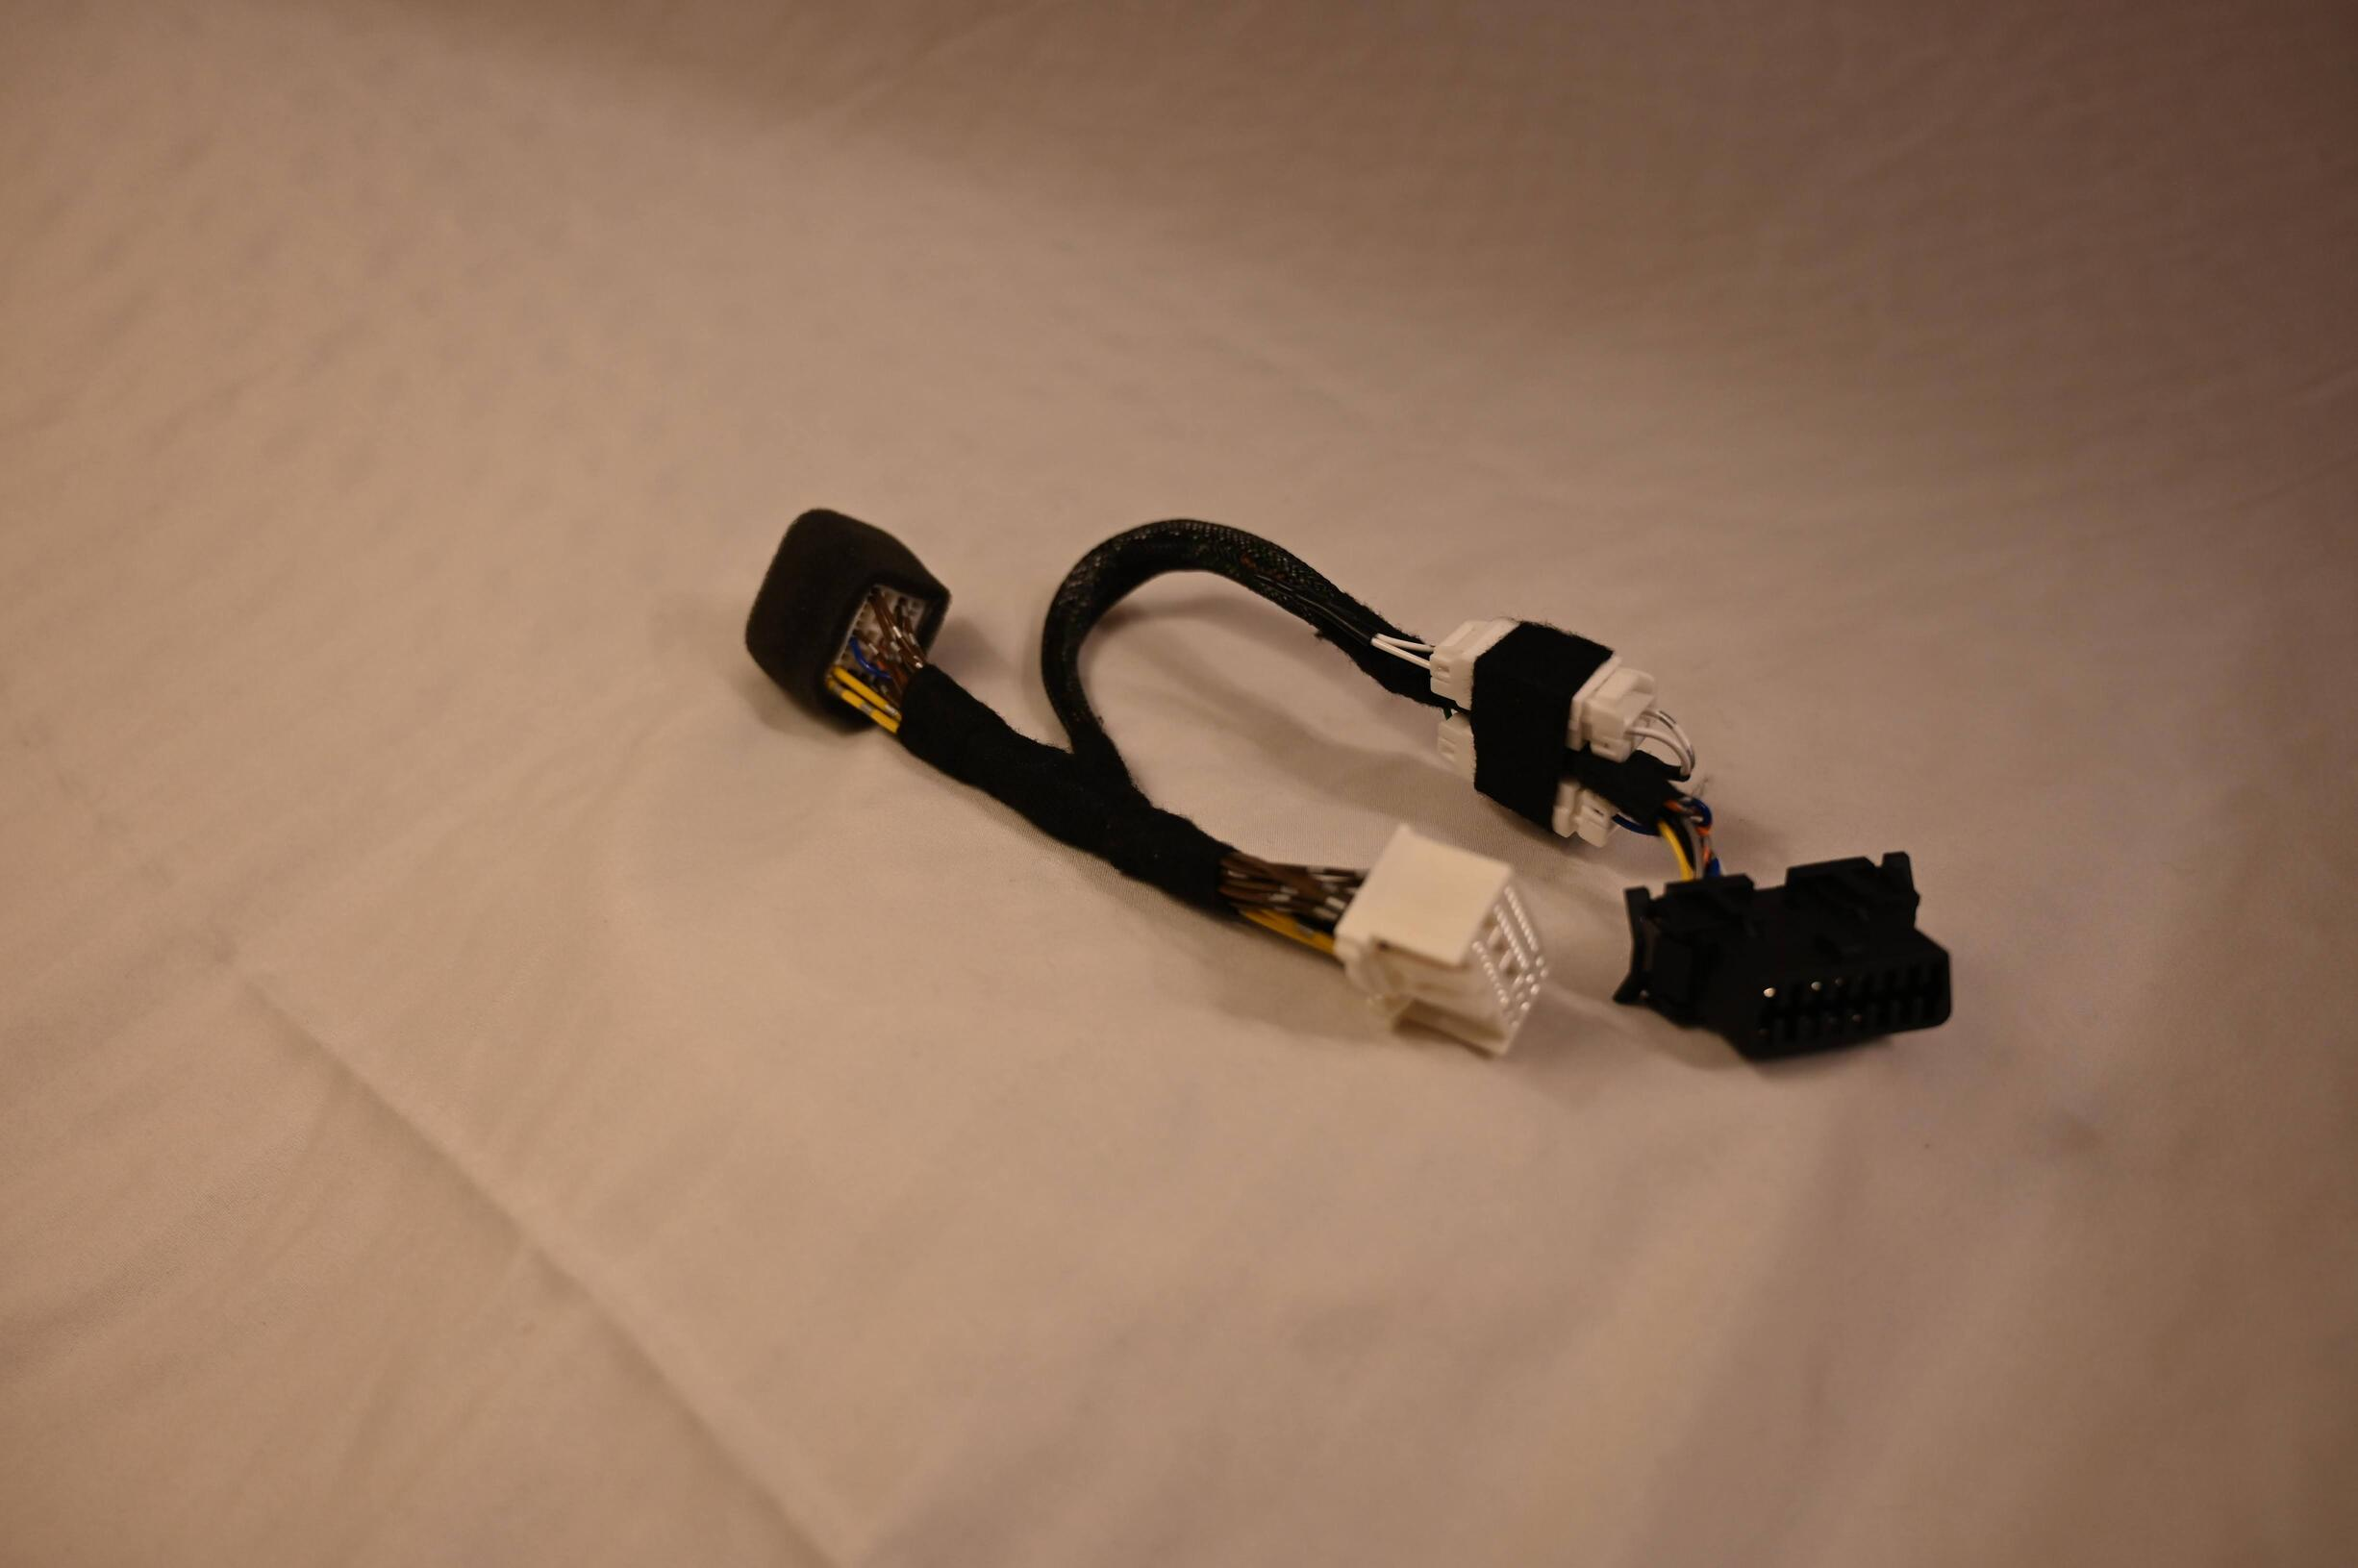
\includegraphics[height=1.95in]{../../../harnesses/head_unit_MITM/photos/whole_harness.jpg} } \\
%   \subfloat[]{\label{subfig:overview:trim}
%   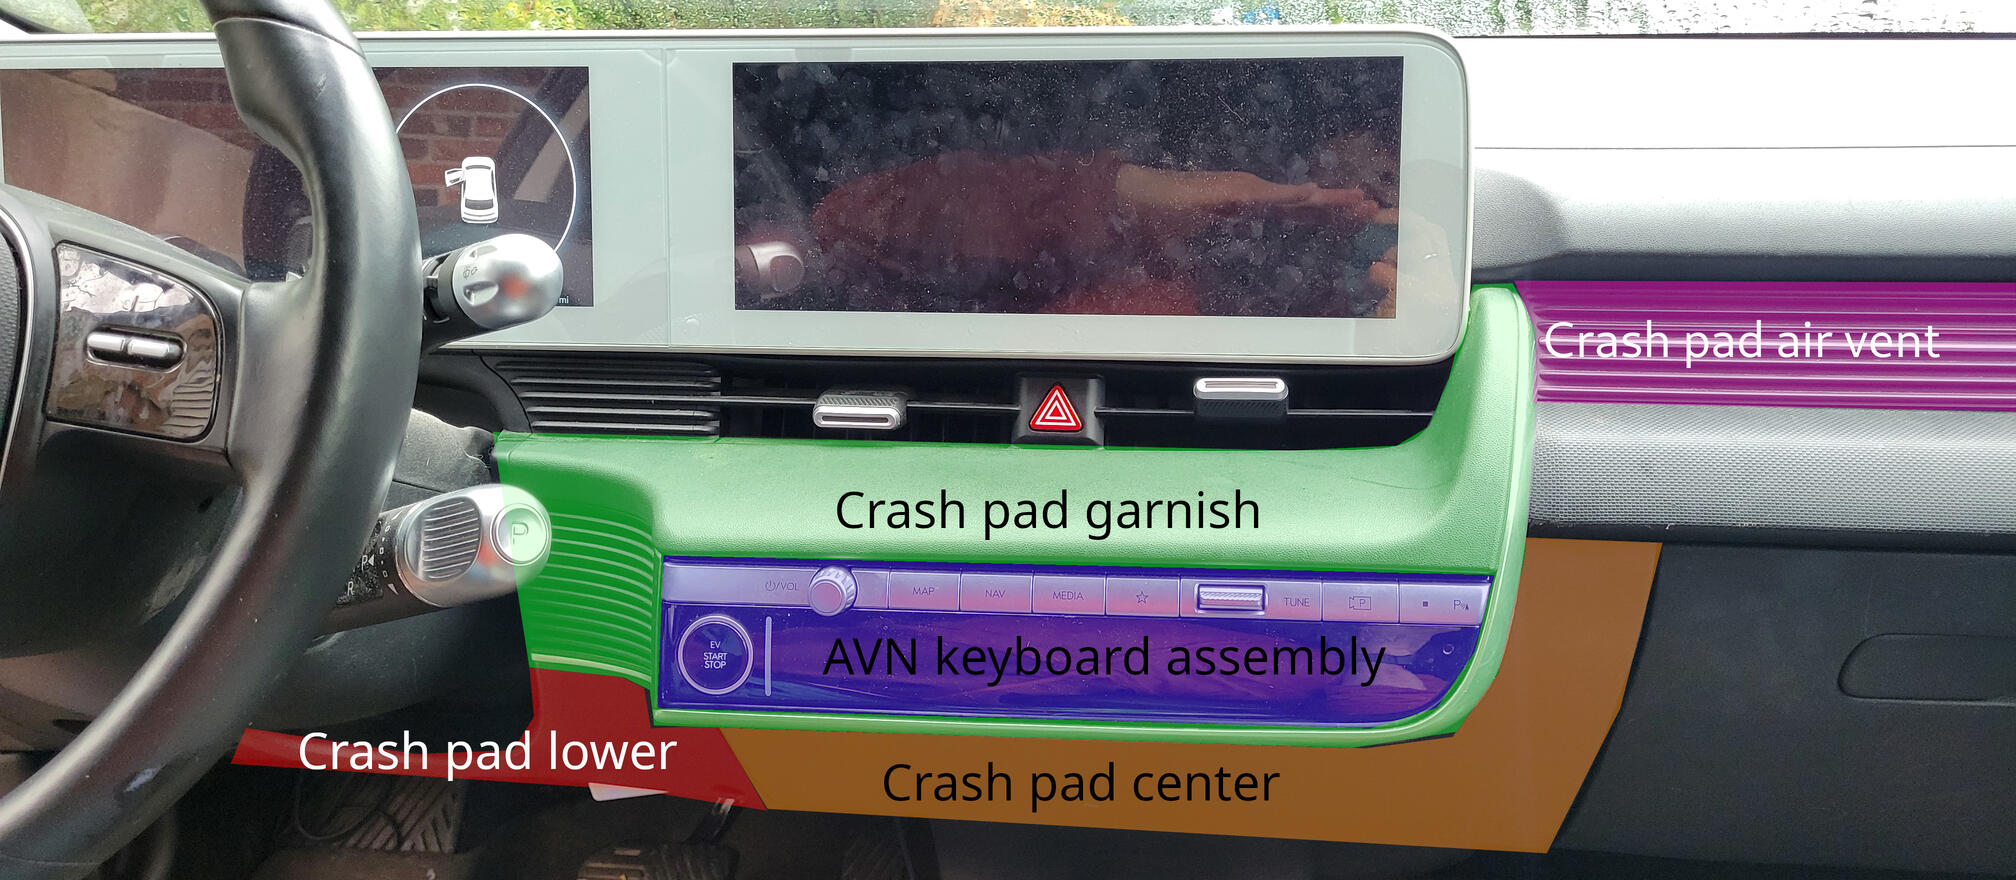
\includegraphics[width=6in]{photos/overview_labeled.jpg} }
%    \caption{(a) Man-in-the-middle harness. (b) Overview of trim panels involved. \label{fig:overview}}
% \end{figure}

\section{Introduction}
Ce guide décrit les étapes d'installation du faisceau CAN sélectionnable dans une ICU Ioniq 5. Voir aussi \href{https://github.com/dragz/explorationsincarhacking/blob/main/articles/getting_past_the_secure_gateway/getting_past_the_secure_gateway.md}{ces instructions} sur l'identification et l'accès au connecteur ICU-H.

Outils nécessaires :
\begin{enumerate}
  \item Douille de 10 mm ou clé à molette pour batterie 12 V
  \item Ciseaux
\end{enumerate}

Composants du kit :
\begin{enumerate}
  \item Faisceau CAN sélectionnable
  \item WiCAN
  \item Support de montage OBD de 60 mm
  \item Ruban adhésif double face de 70 mm (deux pièces incluses pour la redondance)
  \item 4 attaches zippées
\end{enumerate}

\section{Étape 1 : Retirez la borne négative 12 V} \label{sect:0}
Tout d’abord, débranchez toujours la batterie 12V avant de retirer les connecteurs électriques ! Le retrait d'un connecteur électrique sous tension pourrait provoquer une décharge et détruire un connecteur ou un calculateur dans votre voiture.

Instructions étape par étape :
\begin{enumerate}
  \item Capot ouvert (Figure \ref{subfig:12V:hood})
  \item Porte-bagages ouvert 
  \item Retirez le panneau couvrant 12 V (Figure \ref{subfig:12V:panel})
  \item Desserrez l'écrou du côté négatif avec une douille de 10 mm (Figure \ref{subfig:12V:nut})
  \item Retirez la borne négative (Figure \ref{subfig:12V:terminal})
\end{enumerate}

\begin{figure}[h]
  \subfloat[]{\label{subfig:12V:hood}
  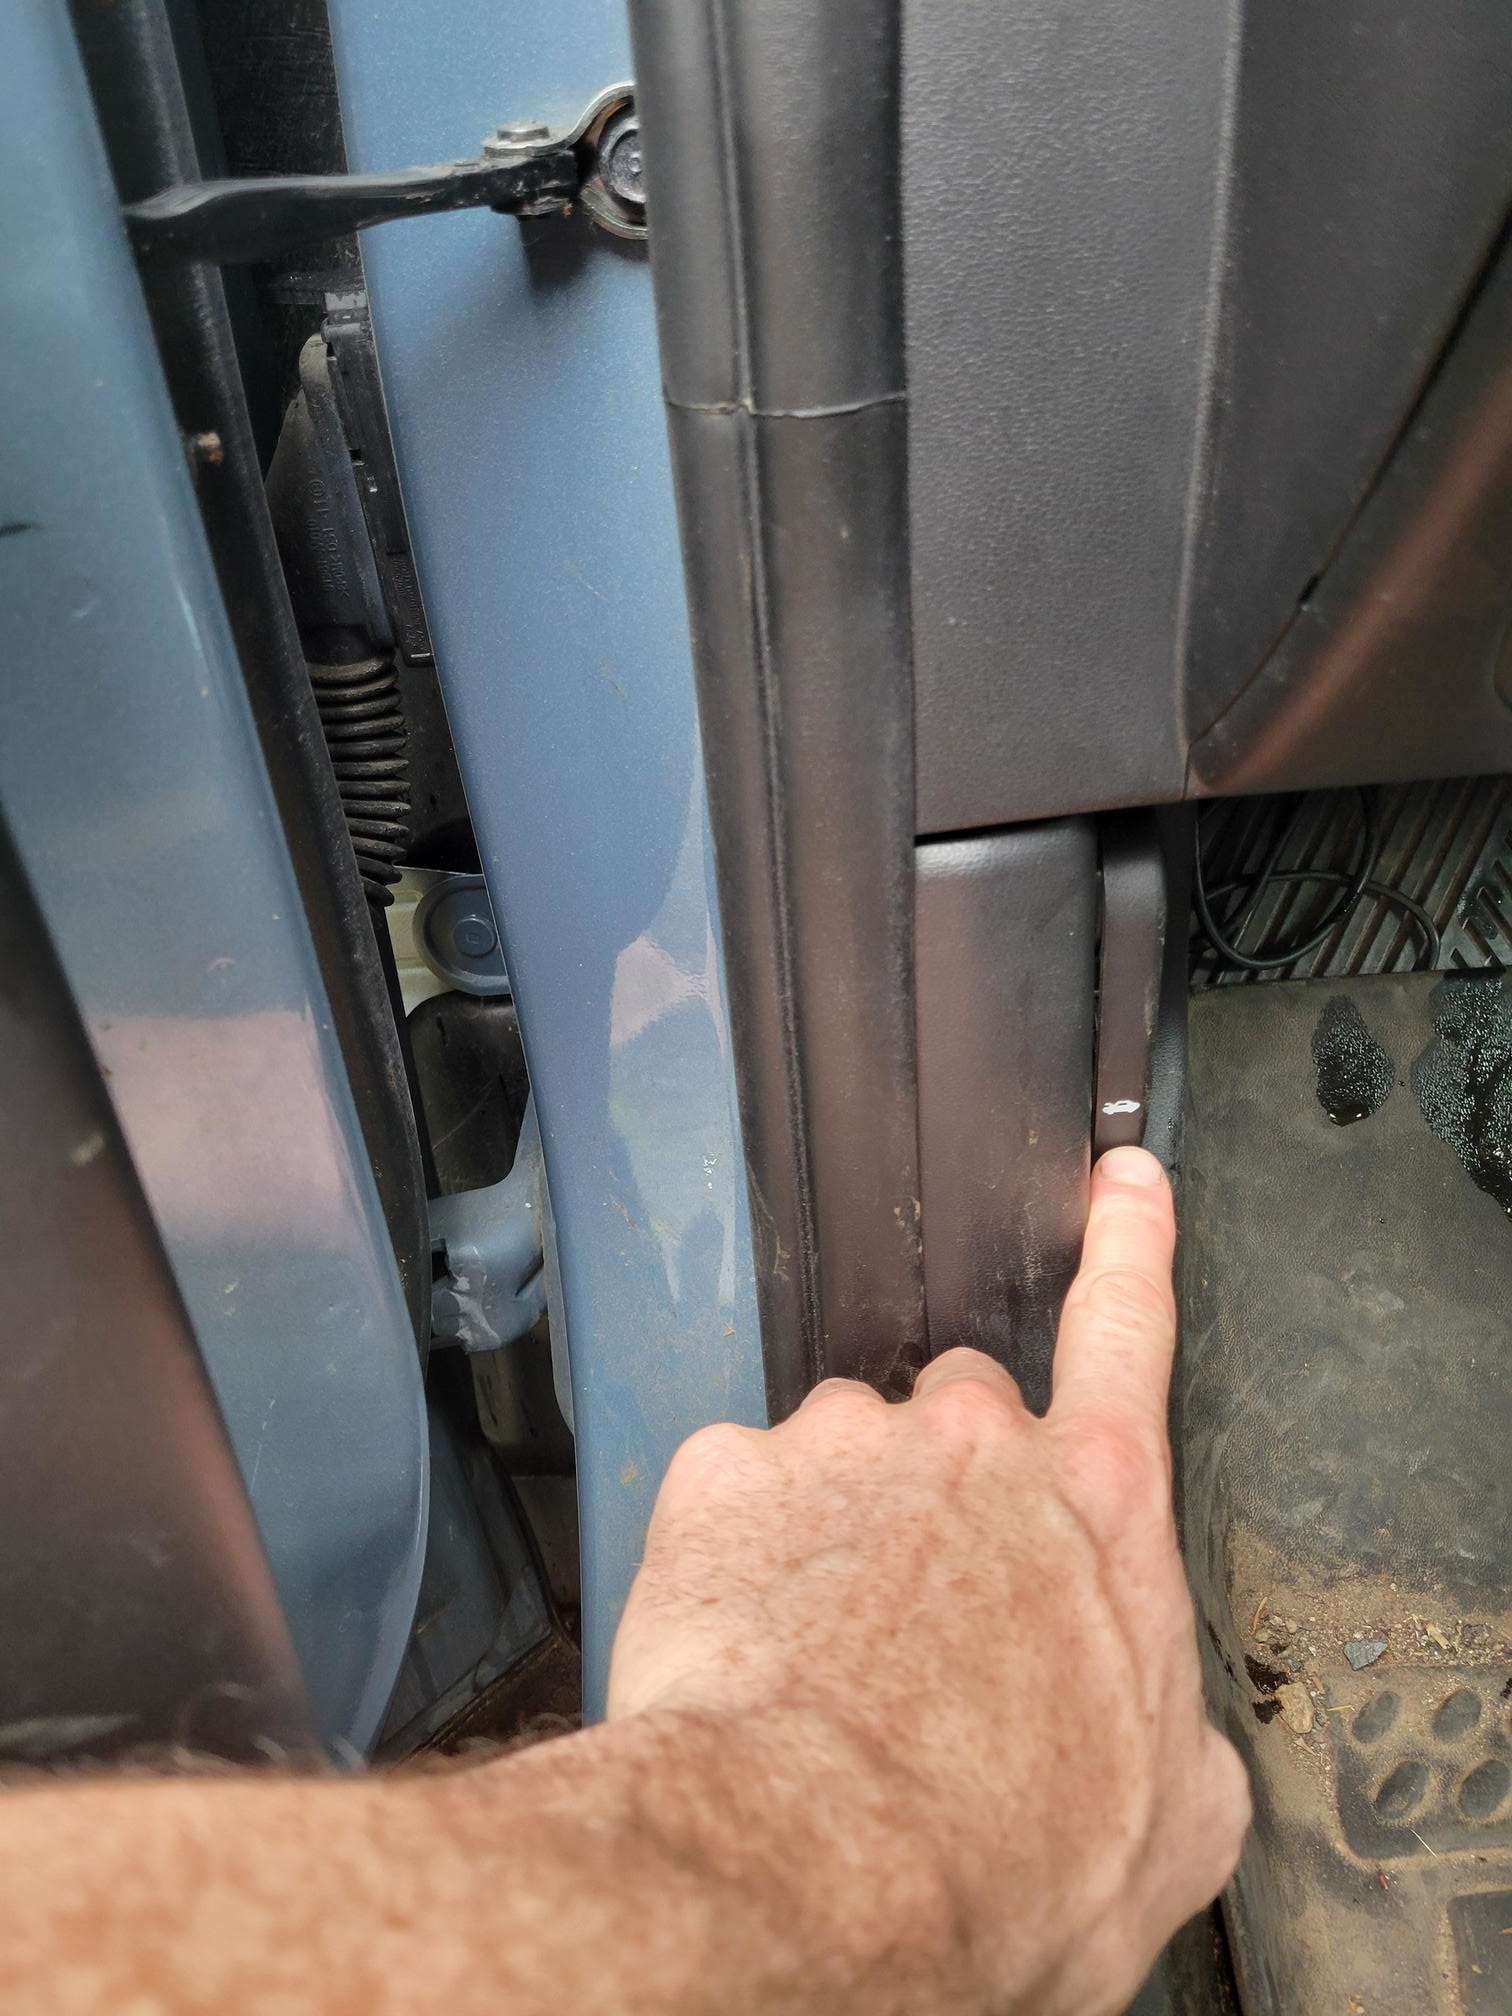
\includegraphics[height=1.5in]{photos/open_hood.jpg} } 
  \subfloat[]{\label{subfig:12V:panel}
  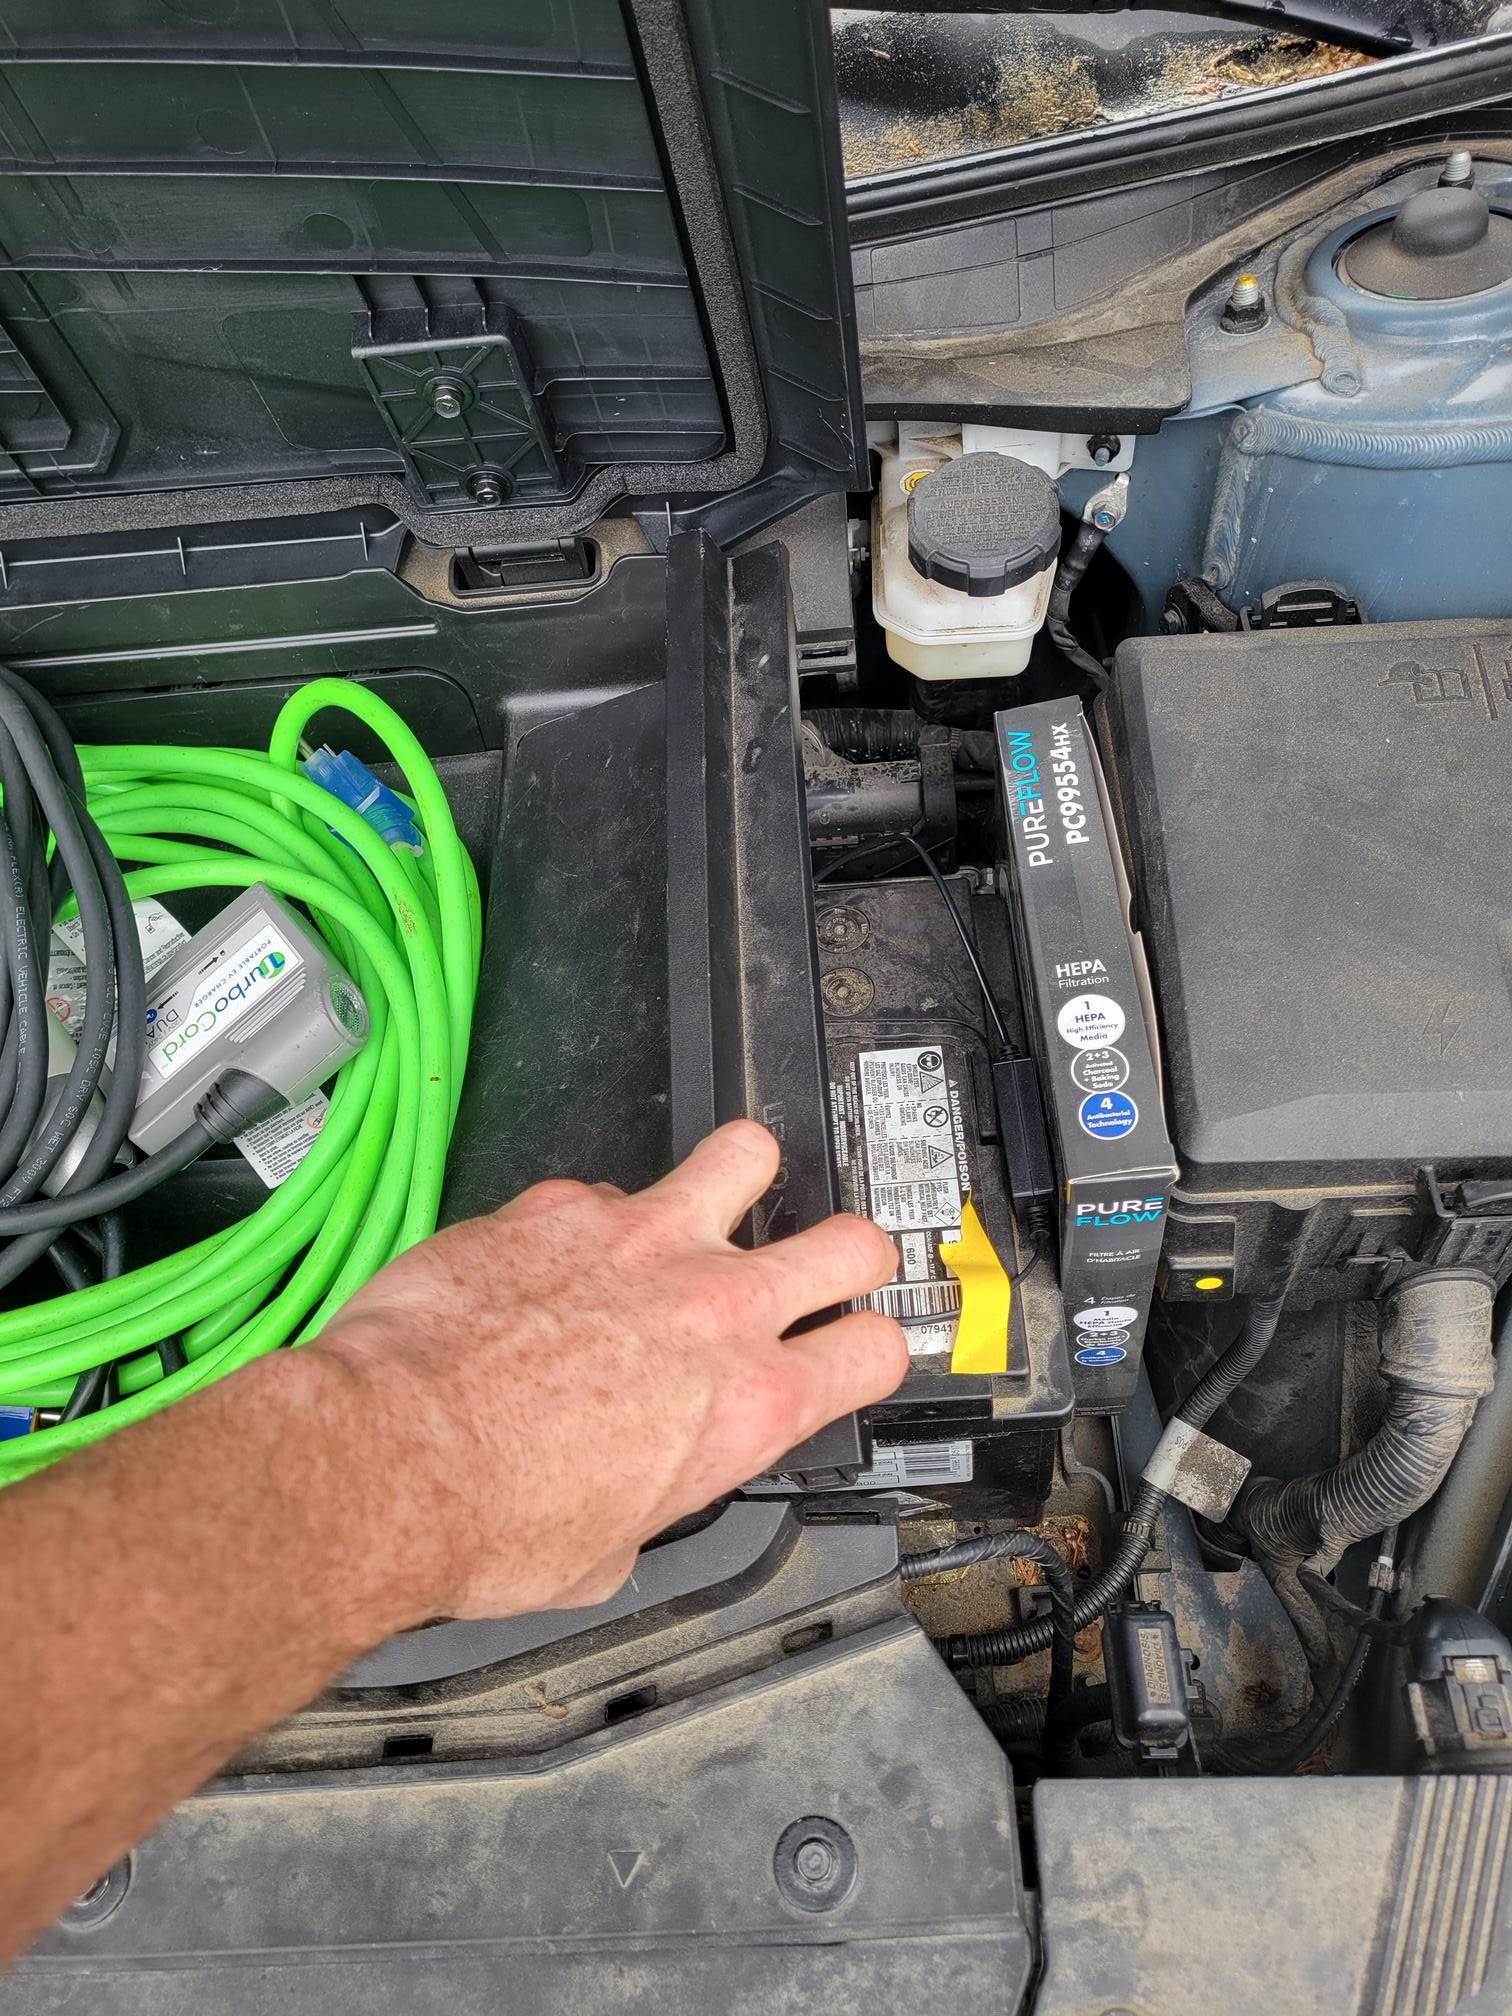
\includegraphics[height=1.5in]{photos/remove_panel.jpg} }  \\
  \subfloat[]{\label{subfig:12V:nut}
  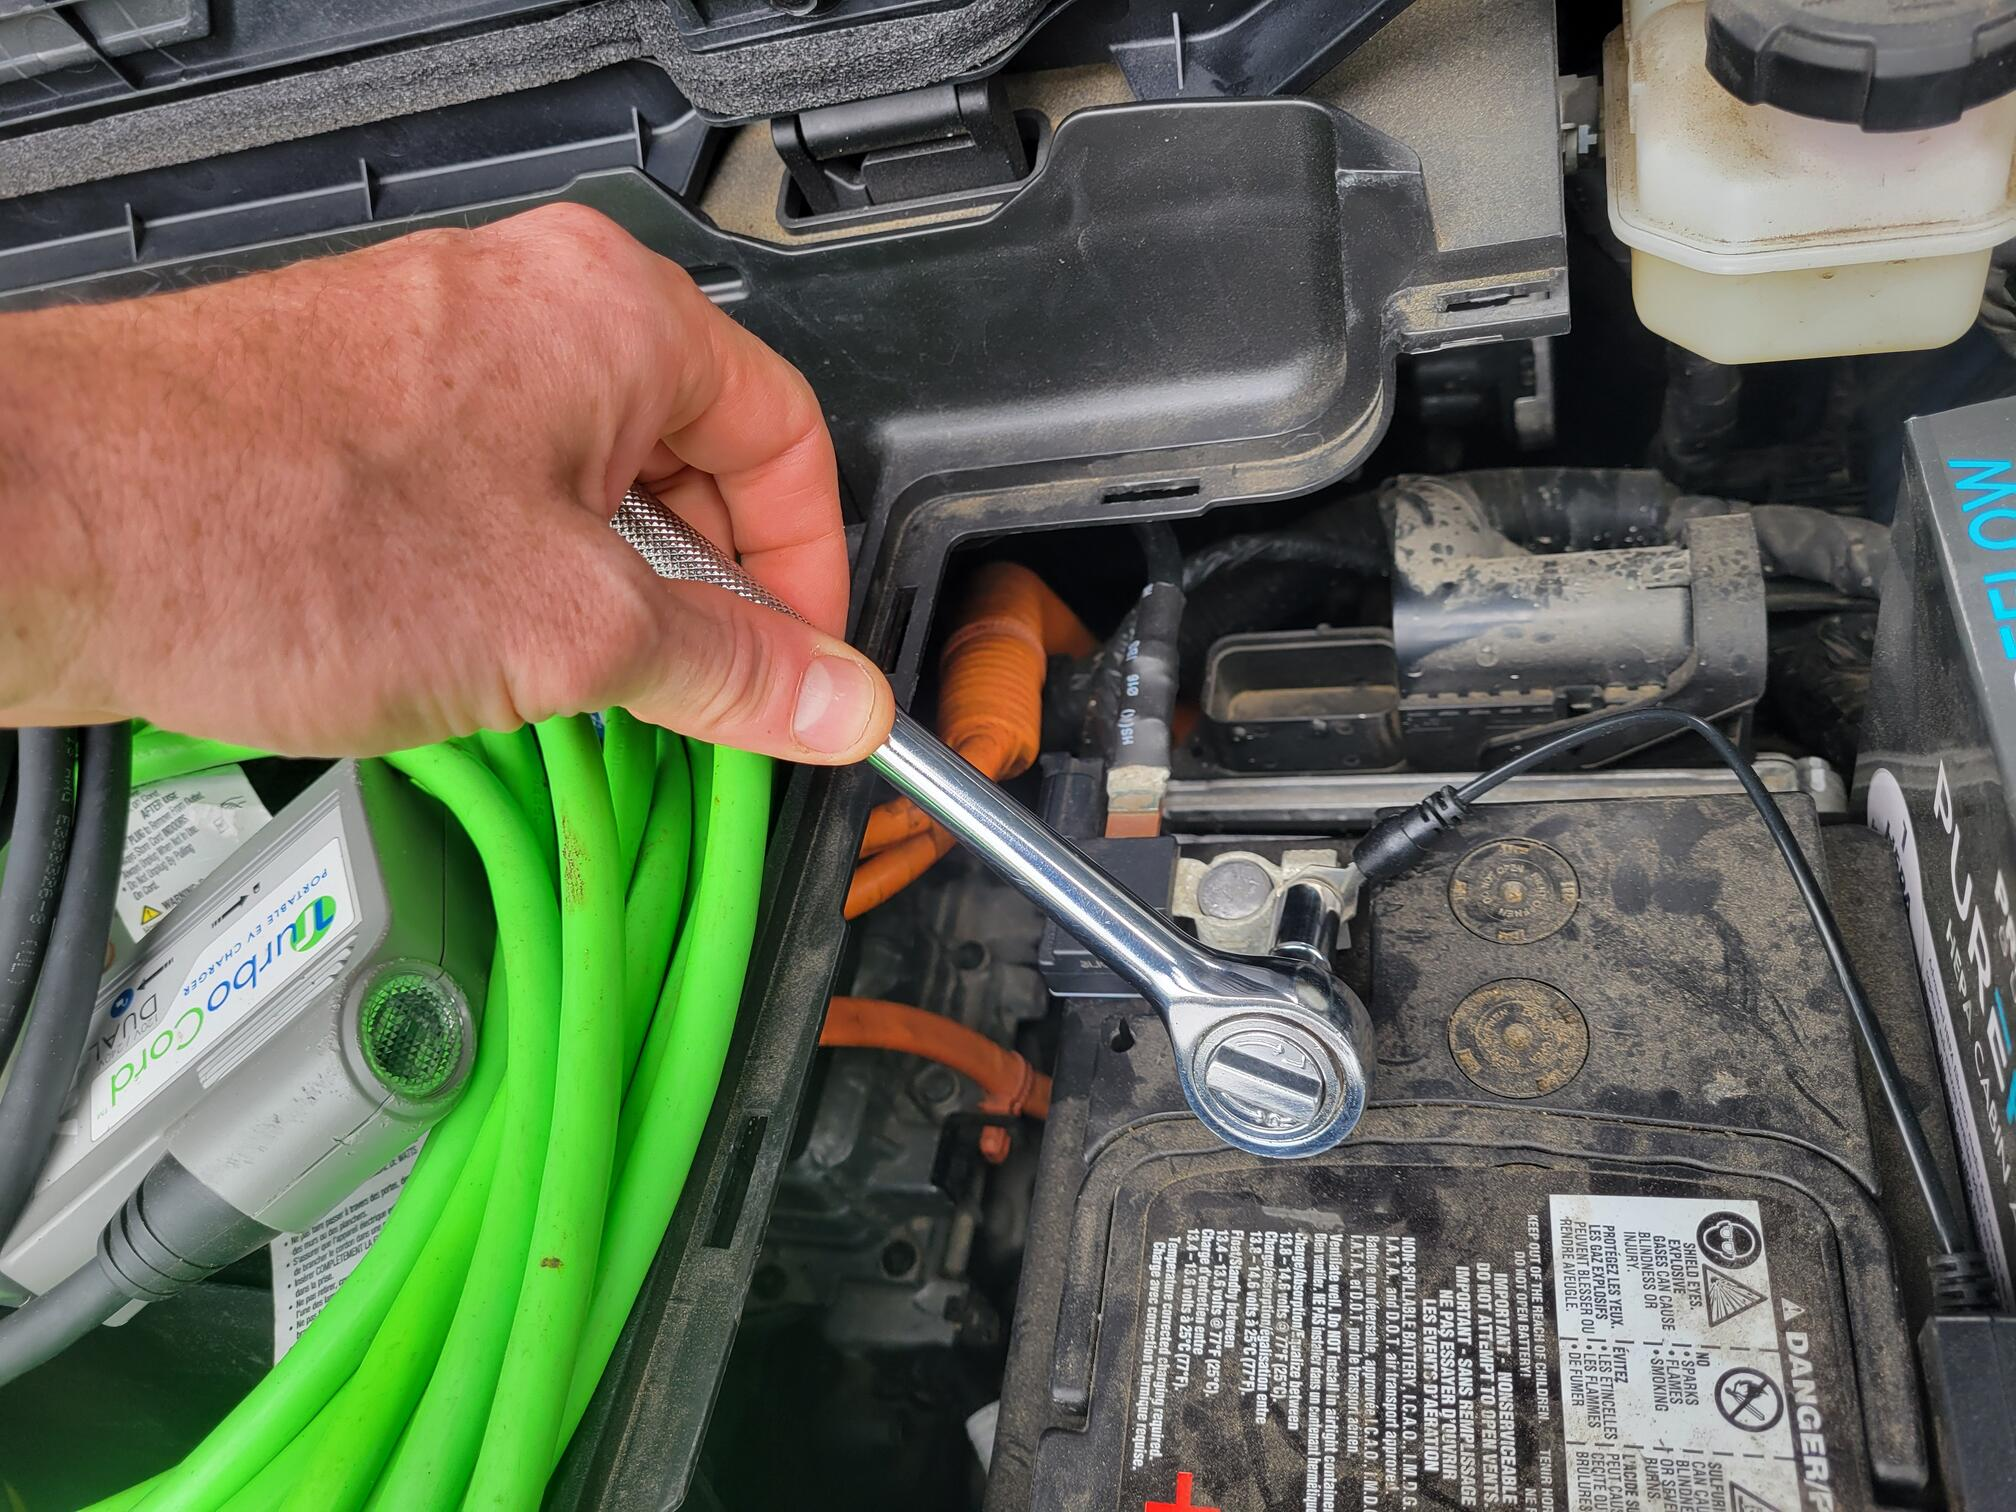
\includegraphics[height=1.5in]{photos/loosen_nut.jpg} } 
  \subfloat[]{\label{subfig:12V:terminal}
  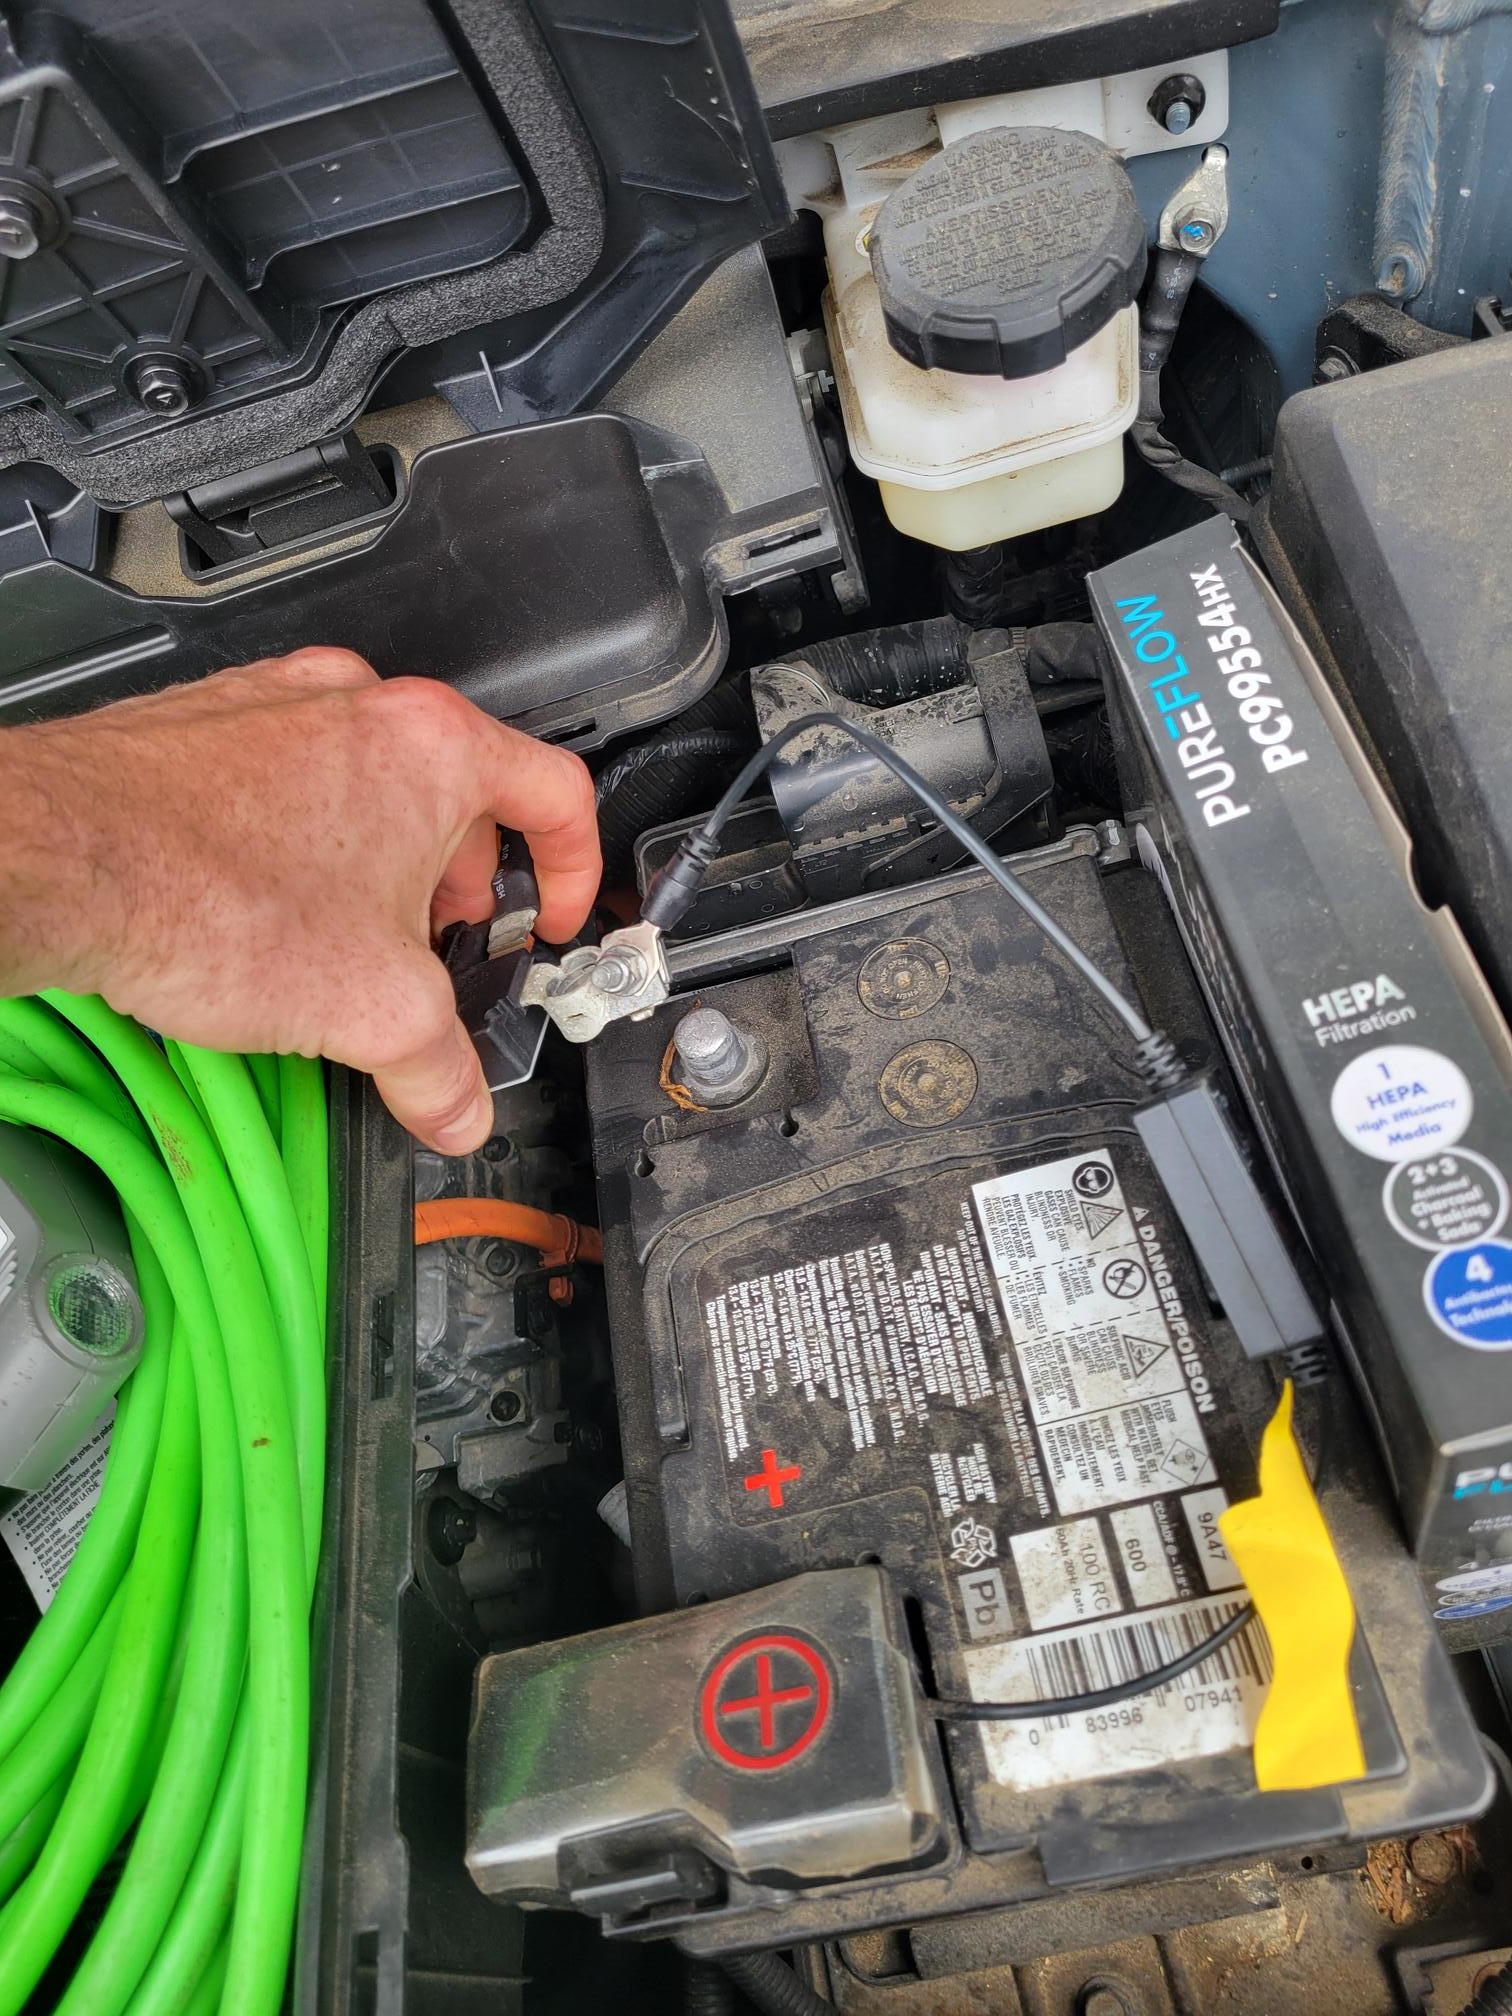
\includegraphics[height=1.5in]{photos/disconnect_terminal.jpg} } 
   \caption{(a) Ouvrez le capot. (b) Retirez le panneau recouvrant 12 V. (c) Desserrez l'écrou sur la borne négative. (d) Retirez la borne négative. \label{fig:12V}}
\end{figure}

\section{Étape 2 : Installation du harnais} \label{sect:2}
Cette étape couvrira l’installation du harnais dans l’USI. 

Instructions étape par étape :
\begin{enumerate}
  \item (Facultatif) Supprimez ICU-H après \href{https://github.com/dragz/explorationsincarhacking/blob/main/articles/getting_past_the_secure_gateway/getting_past_the_secure_gateway.md}{ces instructions}
  \item Installez le robinet à fusible dans le connecteur de rechange 2 pour un fonctionnement permanent, ou dans le connecteur de rechange 1 pour un fonctionnement avec la voiture (Figure \ref{subfig:harness:fusetap})
  \item Retirez le connecteur ICU-H (Figure \ref{subfig:harness:ICU-H})
  \item Insérez le côté femelle du harnais dans l'unité de soins intensifs 
  \item Insérez le connecteur femelle que vous avez retiré dans le côté mâle du faisceau. 
  \item Montez le support sur le côté du connecteur bleu, de sorte que la face OBD pointe vers le bas (Figure \ref{subfig:harness:obd_mount})
  \item Insérez le port OBD dans le support
  \item Insérez WiCAN dans le port OBD
\end{enumerate}

\begin{figure}[h]
  \subfloat[]{\label{subfig:harness:fusetap}
  \includegraphics[height=1.5in,angle=0]{photos/fuse_tap_in_wrong.jpg} } 
  \subfloat[]{\label{subfig:harness:ICU-H}
  \includegraphics[height=1.5in,angle=0]{photos/icu-h_harness_in.jpg} }  
  \subfloat[]{\label{subfig:harness:obd_mount}
  \includegraphics[height=1.5in,angle=0]{photos/obd_mounted_icuh.jpg} } 
   \caption{(a) Robinet à fusible doublé avec robinet à fusible de la dashcam sur la pièce de rechange 2. Notez que cela ne fonctionnera pas comme illustré et nécessite un deuxième fusible sur le robinet à fusible inférieur. (b) ICU-H (flèche verte) avec harnais installé ; connecteur de faisceau mâle (flèche rouge) accouplé au connecteur femelle d'origine. (c) Port OBD monté sur support. \label{fig:harness}}
\end{figure}

\section{Étape 3 : Nettoyer} \label{sect:4}
Rebranchez la borne négative de la batterie 12 V. Le WiCAN devrait immédiatement afficher une lumière bleue. \href{https://meatpihq.github.io/wican-fw/config/wifi}{Changez votre mot de passe WiCAN !}. Vous pouvez connecter votre WiCAN directement en trouvant un réseau WiFi nommé 'WiCAN\_xxxxxxx' et je vais à \href{http://192.168.80.1/}{http://192.168.80.1/} dans votre navigateur.
\appendix 
\bibliographystyle{apsrev4-1}
\bibliography{stemh_model}{}
\end{document}